\documentclass{article}

\usepackage{amsmath, tikz}

% Opening
\title{Drone Package Delivery}
\author{Akash Narayanan}
\date{}

\begin{document}

    \maketitle

    \section{Introduction}
    Suppose you are a recently-hired Amazon employee and you are practicing
    using the delivery drone. In one practice run, the drone starts 5 miles east
    of your home and you aim to fly it directly back home. The drone is
    programmed to travel directly towards your home at a speed of \textbf{b}
    mph. However, there is a wind blowing north at a constant \textbf{w} mph.
    Assuming the drone flies at a constant height, we consider how to construct
    a system of differential equations for this situation along with methods for
    modeling and visualizing the drone's trajectory.

    Our approach involves forming a parametric curve to represent the drone's
    trajectory, using the information about the velocity the drone experiences
    at various points to derive information about it's instantaneous change in
    position. We then use this information with modern numerical methods for
    closely approximating solutions to differential equations which may not have
    analytical solutions.

    \section{Analysis}
    We start by visualizing the problem on the 2D plane. We can do so since the
    drone always flies at the same height. Let the origin represent your home
    and the drone will be represented by a point.

    \begin{figure}[h]
        \centering
        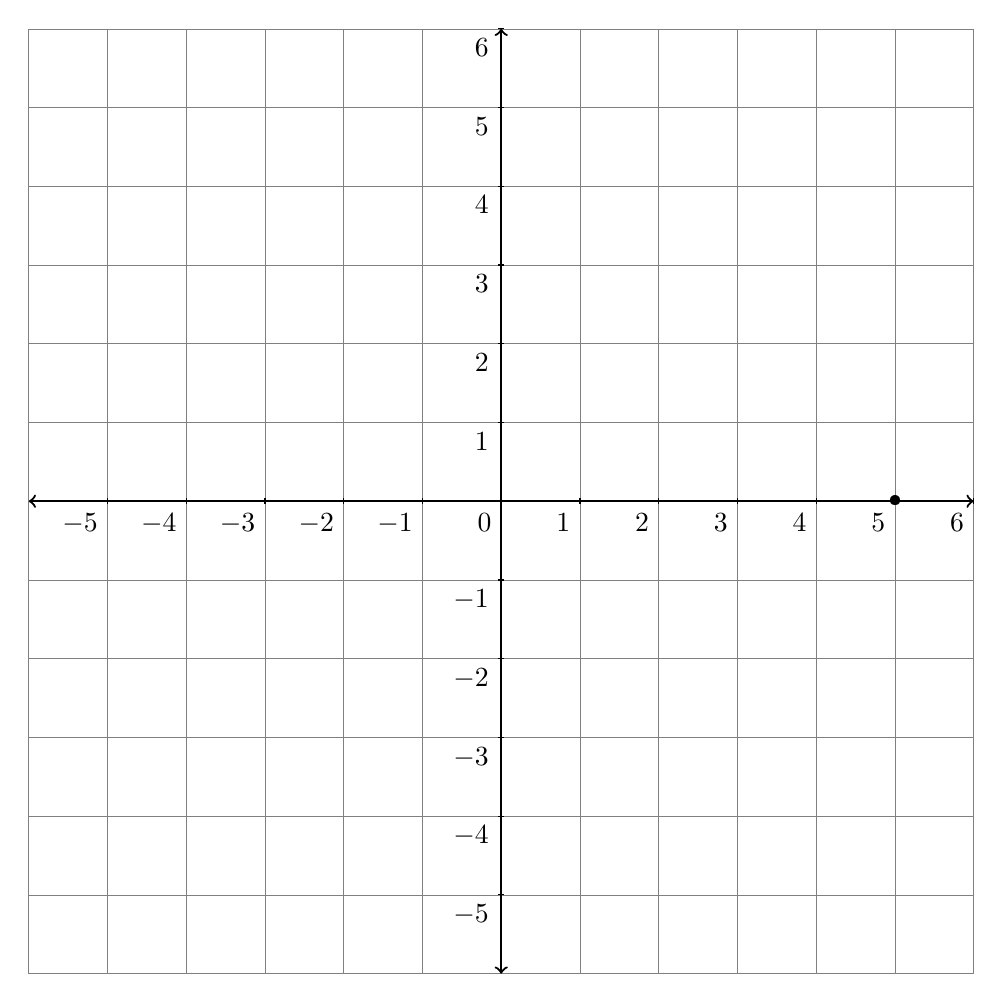
\begin{tikzpicture}
            \draw[step=1cm,gray,very thin] (-6, -6) grid (6, 6);
            \draw[thick, <->] (-6, 0) -- (6, 0);
            \draw[thick, <->] (0, -6) -- (0, 6);
            \foreach \x in {-5, -4, -3, -2, -1, 0, 1, 2, 3, 4, 5, 6}
                \draw (\x cm, 1pt) -- (\x cm, -1pt) node[anchor=north east] {$\x$};
            \foreach \y in {-5, -4, -3, -2, -1, 1, 2, 3, 4, 5, 6}
                \draw (1pt, \y cm) -- (-1pt, \y cm) node[anchor=north east] {$\y$};
            \node at (5, 0) {\textbullet};
        \end{tikzpicture}
    \end{figure}
\end{document}
